\input{../YKY-preamble.tex}

\usepackage{xeCJK}
\setCJKmainfont[BoldFont=SimHei,ItalicFont=KaiTi]{SimSun}
\usepackage{color}
\usepackage{hyperref}
\usepackage{mathtools}

\title{Neural representations}
\author{YKY}

\begin{document}
\maketitle

This is a cartoon diagram that may help our thinking, but is not an accurate depiction of technical details:
\begin{equation}
\vcenter{\hbox{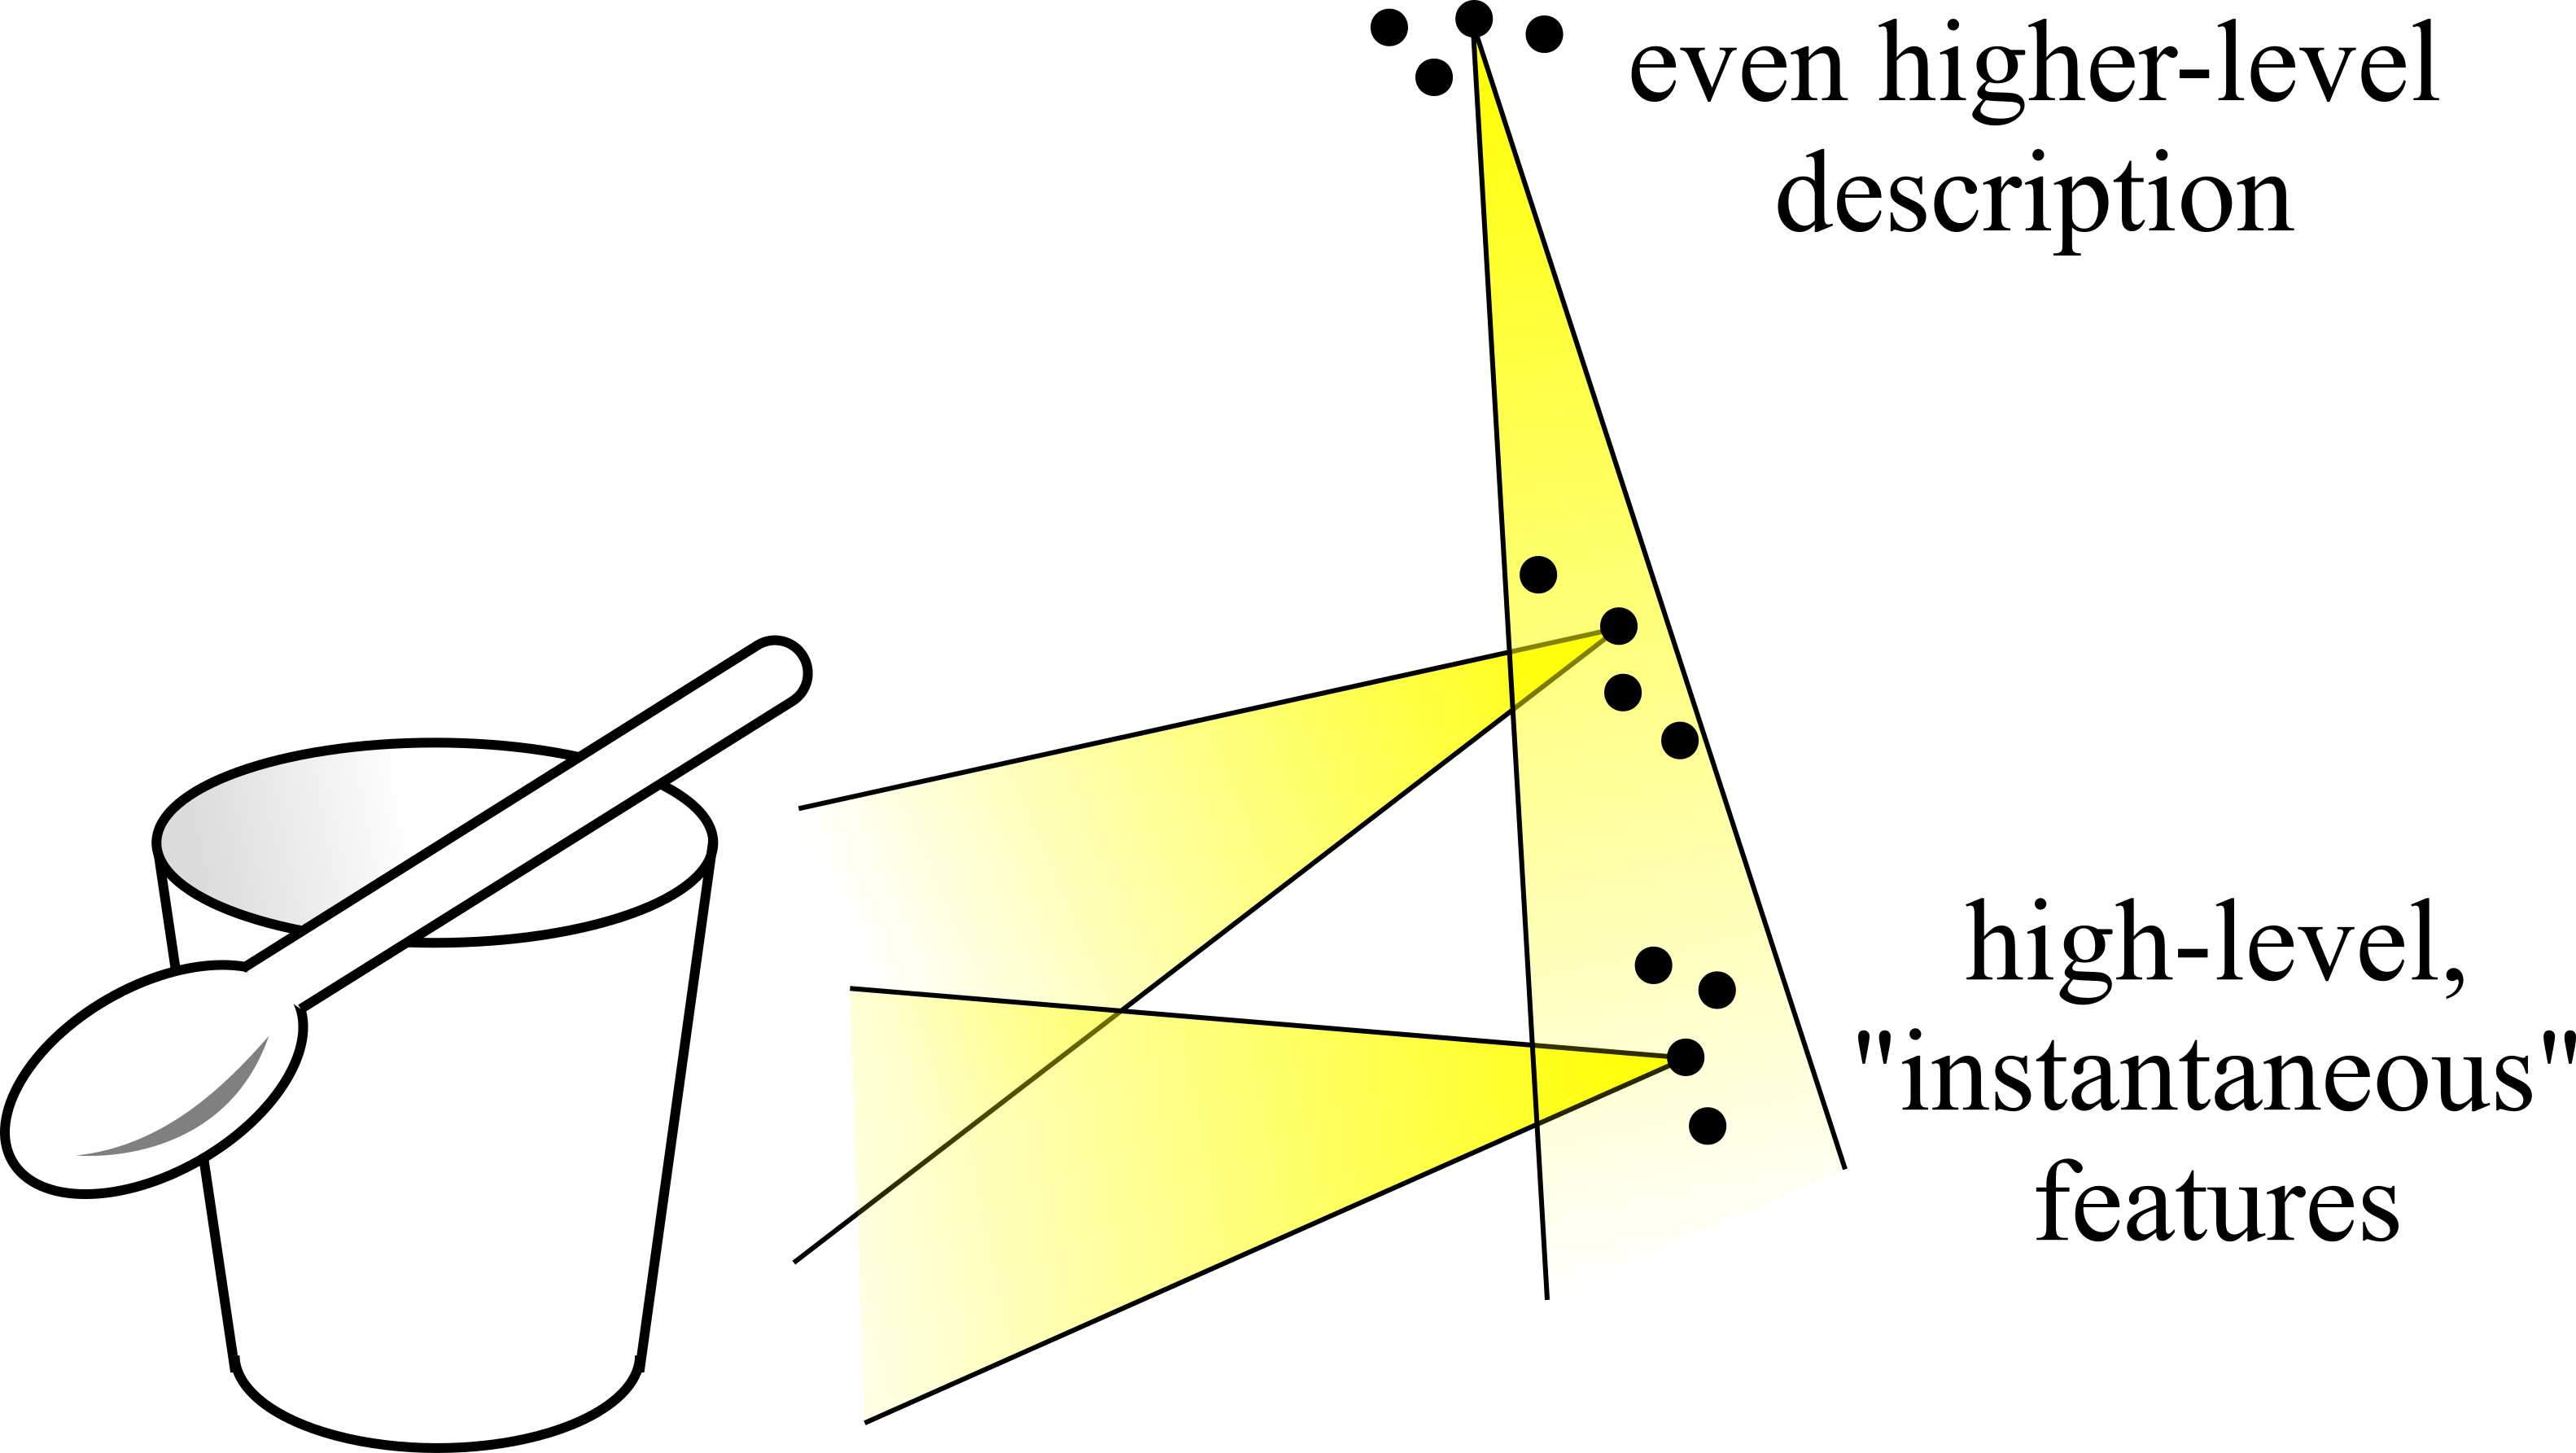
\includegraphics[scale=0.7]{neural-representation.png}}}
\end{equation}

\section{Model vs symbolic propositions}

亦即是说,要避免「匙羹在杯上」这个符号串

But there is a reckoning of the spoon, and of the glass, etc, probably represented by numerous features, and which are also different from the decomposition-of-spoon features.

The reckoning of "on-top" and its decomposition, together describe this particular instance of ``on-top''.  So far so good. 

Each concept is represented by a number of highest-level representatives and their decompositions (constituents).

\section{Question 1: How do features ``stick together'' for different propositions?}

In vision, low-level visual features are ``positional''.  When the scene becomes a more abstract / complex scenario, the representation is no longer spatial.  Different entities may be represented as \textbf{temporal sequences}, where each instant of a sequence contains features that ``stick together''.

For example:  John loves Mary and Mary doesn't love John.  This could be represented by a temporal sequence of 2 components.  The first component represents ``John loves Mary''.  (Each component itself has a distributive representation)

It seems that each ``component'' in the temporal sequence corresponds roughly to a \textbf{proposition} in logic, even though this proposition can be rather complex.  In logic-based AI, this complex proposition may itself be decomposed into smaller propositions (as logic formulas).

The \textbf{commutativity} of logical conjunctions ($A \wedge B \Leftrightarrow B \wedge A$) can be achieved in the brain as the temporal sequence forms a ``loop''.  The exact mechanism that maintains such a loop in the working memory is still unclear (to me at least) but is not essential for our purposes here, which is the design of AGI.

\section{Question 2: What are transition mappings like and how do they handle variable substitutions?}

If John loves Mary but Mary doesn't love John then John would be unhappy.

How does ``John'' appear in the conclusion component?

A temporal sequence seems to describe a complex model.  Multiple temporal components in the sequence may participate in a logical deduction step.  The inference may be carried out using a ``hidden'' state that condenses information in the temporal sequence.

The output ``john'' is also a bunch of neural features, with distributive decompositions.

In other words, the macro concept ``John'' may need to be transferred from one temporal component to another.  This is required because the objects inside various components are not the same, thus the temporal  components need to be \textbf{separated} in time.  The need to maintain this separateness is essential if the system has to \textbf{re-use} neural features.

So the ``variable substitution'' has to move across such boundaries.  Also the transfer is of \textbf{macro} concepts, which seems costly and thus unlikely to exist in the brain.  Or perhaps the temporal separation is with respect to \textbf{objects}? 

But it is not necessary that neural features represent either macro objects or relations.  They may represent propositions.  Then the question is how to use a limited number of features to describe a virtually limitless set of possible propositions?  In symbolic logic this is achieved via the \textbf{compositionality} of concepts or predicates.

Any large number of features may describe the set of possible worlds.  

The logical encoding does not seem to increase or decrease the information content of the representation, measured in bits.

And if this is true, why do we bother to design a particular encoding, rather than just using the ``free'' encoding?

But if the hidden state has structure we may be able to impose inductive bias on the learning algorithm.

What we need to learn is the transition map from state to state.  We already know that permutation symmetry greatly reduces the degrees of freedom of this map.

It seems obvious that neural features are propositions.  But neural features may combine together to form more complex propositions.  The latter level may be the more important aspect of the structure of the KR.



\end{document}